\documentclass{report}
\usepackage{homework}
\solstrue

\renewcommand{\hmwkTitle}{Homework 7}
\usepackage{booktabs}
\usepackage{mathtools}
\usepackage{tikz}
\usepackage{multirow}

\newcommand*\circled[1]{\tikz[baseline=(char.base)]{
    \node[shape=circle, draw, inner sep=1pt, 
        minimum height=12pt] (char) {\vphantom{1g}#1};}}

\begin{document}
\mktitle


\newpage
\begin{problem}
    Consider the network shown below, and assume that each node initially knows the costs to each of its neighbors. Consider the distance-vector algorithm and show the distance table entries at node $z$. (Please write down the calculation steps.)
    
    \begin{center}
    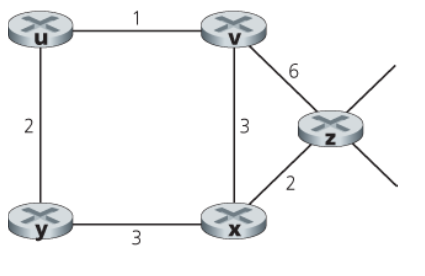
\includegraphics[scale=0.5]{figures/hw7-dv-algorithm.png}
    \end{center}
    
    \medskip
    \begin{answer}{40em}
        \begin{tabular}{c | c c c c c}
            \toprule
            $t$ & $z$ & $v$ & $x$ & $y$ & $u$ \\
            \midrule
            0 & 0 & 6 & 2 & $\infty$ & $\infty$ \\
            1 & 0 & $\min\{6, 2 + 3 = 5\} = 5$ & 2 & $\min\{\infty, 2 + 3 = 5\} = 5$ & $\min\{\infty, 6 + 1 = 7\} = 7$ \\
            2 & 0 & 5 & 2 & $\min\{5, 5 + 1 + 2 = 8\} = 5$ & $\min\{7, 5 + 1 = 6\} = 6$ \\
            \bottomrule
        \end{tabular}
        \newline
        At time $t = 2$, we get
        \newline
        \begin{tabular}{c | c c c c c}
            \toprule
            $t$ & $z$ & $v$ & $x$ & $y$ & $u$ \\
            2 & 0 & 5 & 2 & 5 & 6 \\
            \bottomrule
        \end{tabular}
 
    \end{answer}
\end{problem}





\newpage
\begin{problem}
Consider the network shown below. The costs of all links are initially: c(x,y) = 4, c(x,z) = 50, c(y,w) = 1, c(z,w) = 1, c(y,z) = 3. Suppose the distance-vector algorithm introduced in the lecture is used.
\begin{enumerate}
    \item When the distance vector routing is stabilized, router w, y, and z inform their distances to x to each other. What distance values do they tell each other?
    \item Now suppose that the link cost between x and y increases to 60. Can y, z, w settle their optimal distances to x within several iterations? Why or why not?
    \item Will the distance tables eventually reach a stabilized state? Why or why not?
\end{enumerate}
\begin{center}
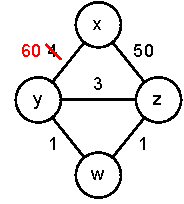
\includegraphics[width=.2\columnwidth]{figures/count-to-infinity.pdf}
\end{center}

\medskip
\begin{answer}{30em}
    \begin{enumerate}
        \item Router y informs w that d(y, x) = 4, z that d(y, x) = 4.
            \newline
            Router w informs y that d(w, x) = 5, z that d(w, x) = 5.
            \newline
            Router z informs y that d(z, x) = 6, w that d(z, x) = 6.
        \item Yes, y, z, w will \textit{eventually} settle their optimal distances to x because the costs are stable.
            Therefore, the new information will be propagated through the network and will eventually
            converge to the optimal distances. Assuming that several iterations means eventually, we can
            see that it will converge to the optimal distances in a finite number of iterations.
        \item The distance tables will eventually reach a stabilized state because they will eventually
            converge to the optimal distances, settling once they do.
    \end{enumerate}
\end{answer}
\end{problem}


\newpage
\begin{problem}
Consider the network shown below.
Suppose AS3 and AS2 are running OSPF for their intra-AS routing protocol.
Suppose AS1 and AS4 are running RIP for their intra-AS routing protocol.
Suppose eBGP and iBGP are used for the inter-AS routing protocol.
Initially suppose there is no physical link (the dotted line between 4a and 2c) between AS2 and AS4.

\begin{center}
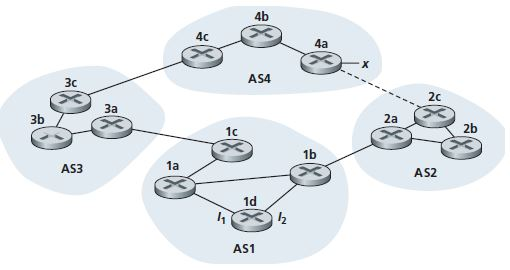
\includegraphics[width=.6\columnwidth]{figures/hw7-q4.jpg}
\end{center}

At some time T, the prefix $x$ appears in AS4, adjacent to the router 4a.
From which routing protocol (OSPF, RIP, eBGP, or iBGP):

\begin{enumerate}
\item Router 4b learns about prefix $x$?
\item Router 3c learns about prefix $x$?
\item Router 1c learns about prefix $x$?
\item Router 1d learns about prefix $x$?
\end{enumerate}



\begin{answer}{30em}
    \begin{enumerate}
        \item RIP
        \item eBGP
        \item eBGP
        \item iBPGP
    \end{enumerate}
\end{answer}
\end{problem}


\newpage
\begin{problem}
Referring to the previous problem, once router 1d learns about $x$ will put an entry $(x, I)$ in its forwarding table:
\begin{enumerate}
\item Will $I$ be equal to $I_1$ or $I_2$ for this entry? Explain why in one sentence.
\item Now suppose that there is a physical link between AS2 and AS4, shown by the dotted line.
Suppose router 1d learns that $x$ is accessible via AS2 as well as via AS3.
Will $I$ be set to $I_1$ or $I_2$? Explain why in one sentence.
\item Now suppose there is another AS, called AS5, which lies on the path between AS2 and AS4 (not shown in the figure).
Suppose router 1d learns that $x$ is accessible via AS2 AS5 AS4 as well as via AS3 AS4.
Will $I$ be set to $I_1$ or $I_2$? Explain why in one sentence.
\end{enumerate}


\begin{answer}{45em}
    \begin{enumerate}
        \item $I_1$ because this is the least cost path towards the gateway router (1c).
        \item $I_2$ because now, the AS-PATH's are the same, meaning we choose the router with the
            least cost path (1d).
        \item $I_1$ because, assuming there is no local preference, we choose the path with the
            shortest AS-PATH.
    \end{enumerate}
\end{answer}

\end{problem}


\newpage
\begin{problem}

Consider the following topology.
The cost metric of a link denotes the one-way propagation delay on the link in msec (assuming the delays are symmetric).
The two ISPs ISP 1 and ISP 2 are peers.
CIDR is used for addressing and BGP is used for inter-domain routing.
Assume that both ISPs always try to enforce hot-potato routing above all other routing policies.
What is the one-way propagation delay between Customer 1 and Customer 2?
Is the routing between two customers symmetric or asymmetric?

\begin{center}
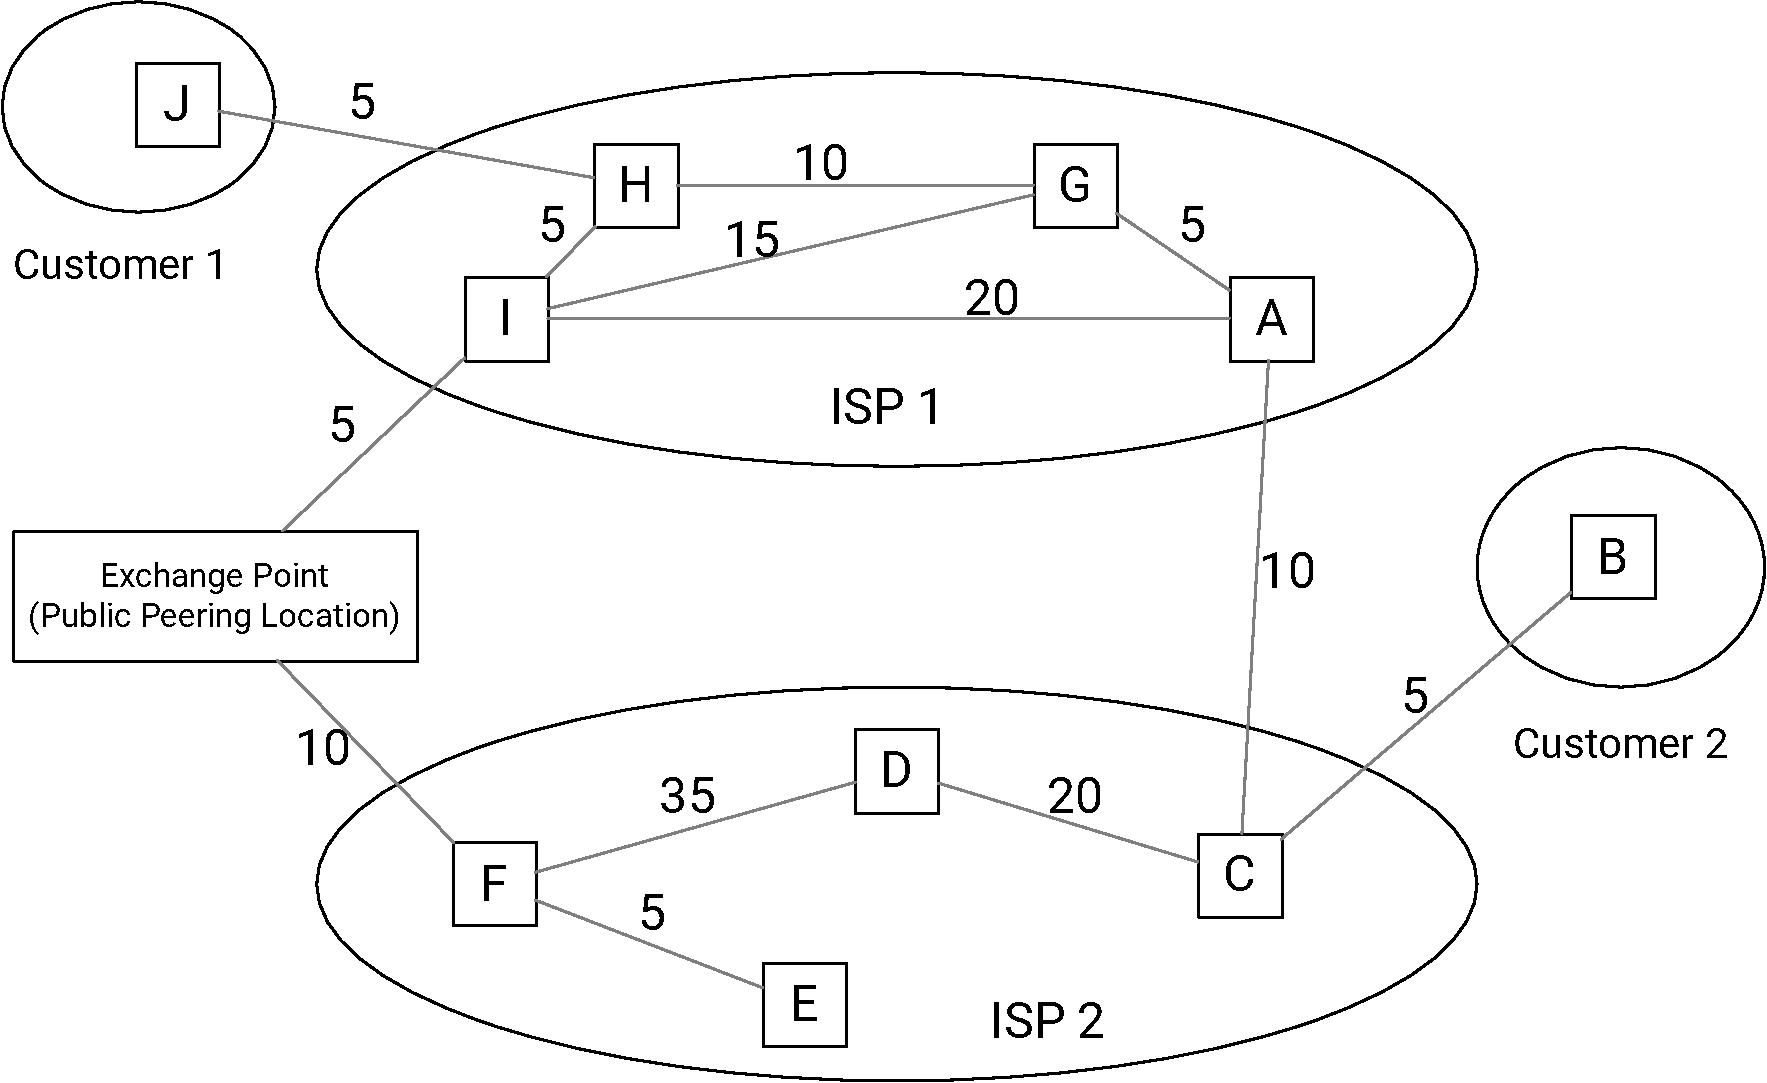
\includegraphics[width=.75\columnwidth]{figures/hw7-3.pdf}
\end{center}

\medskip

\begin{answer}{30em}
    The one way propogation delay between Customer 1 and Customer 2 is:
    \[
        J \overset{5}{\to} H \overset{5}{\to} I \overset{5}{\to} \text{Exchange Point} 
        \overset{10}{\to} F \overset{35}{\to} D \overset{20}{\to} C \overset{5}{\to} B = 85\text{ msec}
    \]

    The routing between the two customers is \textbf{asymmetric} since the one way propagation delay between 
    Customer 2 and Customer 1 is:
    \[
        B \overset{5}{\to} C \overset{10}{\to} A \overset{5}{\to} G 
        \overset{10}{\to} H \overset{5}{\to} J = 35\text{ msec} 
    \]
\end{answer}

\end{problem}


\end{document}
